\documentclass[]{article}
\usepackage{amssymb,amsmath}
\usepackage{ifxetex,ifluatex}
\usepackage{fixltx2e} % provides \textsubscript
\ifxetex
  \usepackage{fontspec,xltxtra,xunicode}
  \defaultfontfeatures{Mapping=tex-text,Scale=MatchLowercase}
  \newcommand{\euro}{€}
\else
  \ifluatex
    \usepackage{fontspec}
    \defaultfontfeatures{Mapping=tex-text,Scale=MatchLowercase}
    \newcommand{\euro}{€}
  \else
    \usepackage[utf8]{inputenc}
  \fi
\fi
\usepackage{color}
\usepackage{fancyvrb}
\DefineShortVerb[commandchars=\\\{\}]{\|}
\DefineVerbatimEnvironment{Highlighting}{Verbatim}{commandchars=\\\{\}}
% Add ',fontsize=\small' for more characters per line
\newenvironment{Shaded}{}{}
\newcommand{\KeywordTok}[1]{\textcolor[rgb]{0.00,0.44,0.13}{\textbf{{#1}}}}
\newcommand{\DataTypeTok}[1]{\textcolor[rgb]{0.56,0.13,0.00}{{#1}}}
\newcommand{\DecValTok}[1]{\textcolor[rgb]{0.25,0.63,0.44}{{#1}}}
\newcommand{\BaseNTok}[1]{\textcolor[rgb]{0.25,0.63,0.44}{{#1}}}
\newcommand{\FloatTok}[1]{\textcolor[rgb]{0.25,0.63,0.44}{{#1}}}
\newcommand{\CharTok}[1]{\textcolor[rgb]{0.25,0.44,0.63}{{#1}}}
\newcommand{\StringTok}[1]{\textcolor[rgb]{0.25,0.44,0.63}{{#1}}}
\newcommand{\CommentTok}[1]{\textcolor[rgb]{0.38,0.63,0.69}{\textit{{#1}}}}
\newcommand{\OtherTok}[1]{\textcolor[rgb]{0.00,0.44,0.13}{{#1}}}
\newcommand{\AlertTok}[1]{\textcolor[rgb]{1.00,0.00,0.00}{\textbf{{#1}}}}
\newcommand{\FunctionTok}[1]{\textcolor[rgb]{0.02,0.16,0.49}{{#1}}}
\newcommand{\RegionMarkerTok}[1]{{#1}}
\newcommand{\ErrorTok}[1]{\textcolor[rgb]{1.00,0.00,0.00}{\textbf{{#1}}}}
\newcommand{\NormalTok}[1]{{#1}}
\usepackage{graphicx}
% We will generate all images so they have a width \maxwidth. This means
% that they will get their normal width if they fit onto the page, but
% are scaled down if they would overflow the margins.
\makeatletter
\def\maxwidth{\ifdim\Gin@nat@width>\linewidth\linewidth
\else\Gin@nat@width\fi}
\makeatother
\let\Oldincludegraphics\includegraphics
\renewcommand{\includegraphics}[1]{\Oldincludegraphics[width=\maxwidth]{#1}}
\ifxetex
  \usepackage[setpagesize=false, % page size defined by xetex
              unicode=false, % unicode breaks when used with xetex
              xetex,
              bookmarks=true,
              pdfauthor={},
              pdftitle={},
              colorlinks=true,
              urlcolor=blue,
              linkcolor=blue]{hyperref}
\else
  \usepackage[unicode=true,
              bookmarks=true,
              pdfauthor={},
              pdftitle={},
              colorlinks=true,
              urlcolor=blue,
              linkcolor=blue]{hyperref}
\fi
\hypersetup{breaklinks=true, pdfborder={0 0 0}}
\setlength{\parindent}{0pt}
\setlength{\parskip}{6pt plus 2pt minus 1pt}
\setlength{\emergencystretch}{3em}  % prevent overfull lines
\setcounter{secnumdepth}{0}


\begin{document}

\section{Creating Geo-Spatial Analysis Grid for PEP and BOSS Surveys}

\subsubsection{12 June 2012}

\subsubsection{EASE-Grid v2.0}

EASE-grid is an abbrevation for \emph{Equal-Area Scalable Earth Grid}.
It is intended to be a versatile format for global-scale gridded data,
specifically remotely sensed data, although it has gained popularity as
a common gridding scheme for other data as well. Data from various
sources can be expressed as digital arrays of varying grid resolutions,
which are defined in relation to one of three possible projections:
Northern and Southern Hemisphere (Lambert's equal-area, azimuthal) and
full global (cylindrical, equal-area). There are two versions of
EASE-Grid; the first was defined in 1992 and has been used for many data
sets, while EASE-Grid 2.0 was defined in 2011 and is recommended for new
data sets.

Original EASE-Grid Format Description
\href{http://nsidc.org/data/ease/ease\_grid.html}{http://nsidc.org/data/ease/ease\_grid.html}

EASE-Grid 2.0 Format Description
\href{http://nsidc.org/data/ease/ease\_grid2.html}{http://nsidc.org/data/ease/ease\_grid2.html}

\subsubsection{PEP Spatial Analysis Grid}

To facilitate geo-spatial analysis of data from the 2012+ BOSS effort a
subset of the EASE-Grid v2.0 will be used. For this purpose, we will
maintain the grid structure used for distribution of SSM/I sea-ice
concentration, but specify only a subset of cells that are relevant to
our study area.

\subsubsection{Getting Started in R}

To get started in R, we'll load in our essential spatial packages

\begin{Shaded}
\begin{Highlighting}[]
\KeywordTok{library}\NormalTok{(rgdal)}
\end{Highlighting}
\end{Shaded}
\begin{verbatim}
## Loading required package: sp
\end{verbatim}

\begin{verbatim}
## Geospatial Data Abstraction Library extensions to R successfully loaded
## Loaded GDAL runtime: GDAL 1.9.0, released 2011/12/29
## Path to GDAL shared files: /Library/Frameworks/GDAL.framework/Versions/1.9/Resources/gdal
## Loaded PROJ.4 runtime: Rel. 4.8.0, 6 March 2012, [PJ_VERSION: 480]
## Path to PROJ.4 shared files: (autodetected)
\end{verbatim}

\begin{Shaded}
\begin{Highlighting}[]
\KeywordTok{library}\NormalTok{(sp)}
\KeywordTok{library}\NormalTok{(rgeos)}
\end{Highlighting}
\end{Shaded}
\begin{verbatim}
## Loading required package: stringr
\end{verbatim}

\begin{verbatim}
## rgeos: (SVN revision 330)
##  GEOS runtime version: 3.3.2-CAPI-1.7.2 
##  Polygon checking: TRUE 
##  WARNING! if you turn polygon checking off, and polygons are
##  not valid in GEOS, you risk losing data as your R session may crash! 
## 
\end{verbatim}

\begin{Shaded}
\begin{Highlighting}[]
\KeywordTok{library}\NormalTok{(raster)}
\end{Highlighting}
\end{Shaded}
\begin{verbatim}
## raster 1.9-92 (1-May-2012)
\end{verbatim}

We will also load up a personal package \texttt{nPacMaps} which provides
US, Russia and Canada as \emph{SpatialPolygons}. The package is
available upon request from JML.

\begin{Shaded}
\begin{Highlighting}[]
\KeywordTok{library}\NormalTok{(nPacMaps)}
\end{Highlighting}
\end{Shaded}
To determine the boundaries of our study area, we need to examine the
SSM/I EASE-Grid cells along with Russia and US land polygons. We'll use
one of the daily SSM/I EASE-Grid GeoTIFF files as a basis for creating
the grid. So, let's download the GeoTIFF from the new
akc-nmml/polar/data directory on the AFSC network and read it into R as
a \emph{RasterLayer} object using the \texttt{raster} package.

\begin{Shaded}
\begin{Highlighting}[]
\NormalTok{tmp <- }\KeywordTok{tempfile}\NormalTok{(}\DataTypeTok{fileext =} \StringTok{".tif"}\NormalTok{)}
\KeywordTok{download.file}\NormalTok{(}\KeywordTok{paste}\NormalTok{(}\StringTok{"file:///Volumes/Polar/Data/Environ/SeaIce/SSMI_SIC/2012/"}\NormalTok{, }
    \StringTok{"nt_20120401_f17_nrt_n.bin.reproj.tif"}\NormalTok{, }\DataTypeTok{sep =} \StringTok{""}\NormalTok{), tmp)}
\CommentTok{# non-mac users will likely need to replace /Volumes/ with //akc-nmml/}
\NormalTok{r <- }\KeywordTok{raster}\NormalTok{(tmp)}
\NormalTok{r}
\end{Highlighting}
\end{Shaded}
\begin{verbatim}
## class       : RasterLayer 
## dimensions  : 480, 480, 230400  (nrow, ncol, ncell)
## resolution  : 25068, 25068  (x, y)
## extent      : -5922823, 6109589, -5874646, 6157766  (xmin, xmax, ymin, ymax)
## coord. ref. : +proj=laea +lat_0=90 +lon_0=0 +x_0=0 +y_0=0 +datum=WGS84 +units=m +no_defs +ellps=WGS84 +towgs84=0,0,0 
## values      : /private/var/folders/42/x3dcnwt91pgdvgdmn_l3gtkh0004p2/T/RtmpwvQXQp/file40f35f3f85bb.tif 
## min value   : 0 
## max value   : 255 
## layer name  : file40f35f3f85bb 
## 
\end{verbatim}

\subsubsection{NSIDC SSM/I GeoTiff Sea-ice Concentration Files}

The coordinate reference system describes the EASE Grid v2.0 projection.
This is an equal area projection based on the Lambert Azimuthal Equal
Area projection and is centered with a latitude of origin at the north
pole and a longitude of origin set to 0 degrees. The nominal cell
dimension is 25km x 25km, however, as is shown above, the actual
dimension is 25.06753km x 25.06753km.

The data within the raster are stored as one-byte values that need to be
decoded. The following text from the
\href{http://nsidc.org/data/docs/daac/nsidc0051\_gsfc\_seaice.gd.html\#paramrange}{NSIDC
website} desribes the coding.

\begin{quote}
Data are stored as one-byte integers representing sea ice concentration
values. The sea ice concentration data are packed into byte format by
multiplying the derived fractional sea ice concentration floating-point
values (ranging from 0.0 to 1.0) by a scaling factor of 250. For
example, a sea ice concentration value of 0.0 (0\%) maps to a stored
one-byte integer value of 0, and a sea ice concentration value of 1.0
(100\%) maps to a stored one-byte integer value of 250. To convert to
the fractional parameter range of 0.0 to 1.0, divide the scaled data in
the file by 250. To convert to percentage values (0\% to 100\%), divide
the scaled data in the file by 2.5.
\end{quote}

\begin{quote}
Data files may contain integers from 0 to 255, as described

\textbf{0 - 250} \ldots{}. Sea ice concentration (fractional coverage
scaled by 250) \textbf{251} \ldots{}\ldots{}.. Circular mask used in the
Arctic to cover the irregularly-shaped data gap around the pole (caused
by the orbit inclination and instrument swath) \textbf{252}
\ldots{}\ldots{}.. Unused \textbf{253} \ldots{}\ldots{}.. Coastlines
\textbf{254} \ldots{}\ldots{}.. Superimposed land mask \textbf{255}
\ldots{}\ldots{}.. Missing data
\end{quote}

So, we need to divide the values 0-250 by 2.5 to represent sea-ice
concentration and either leave the 251-255 values as is or set them to
NA. In this case, we'll set all values above 250 to NA. We can do this
using the \texttt{calc} function within the \texttt{raster} package.

\begin{Shaded}
\begin{Highlighting}[]
\NormalTok{fun <- function(x) \{}
    \KeywordTok{ifelse}\NormalTok{(x < }\DecValTok{251}\NormalTok{, x/}\FloatTok{2.5}\NormalTok{, }\OtherTok{NA}\NormalTok{)}
\NormalTok{\}}
\NormalTok{sic_raster <- }\KeywordTok{calc}\NormalTok{(r, fun)}
\end{Highlighting}
\end{Shaded}
\begin{Shaded}
\begin{Highlighting}[]
\KeywordTok{plot}\NormalTok{(sic_raster, }\DataTypeTok{main =} \StringTok{"Northern Hemisphere SSM/I Sea-Ice Concentration}\CharTok{\textbackslash{}n}\StringTok{01 April 2012"}\NormalTok{)}
\end{Highlighting}
\end{Shaded}
\begin{figure}[htbp]
\centering
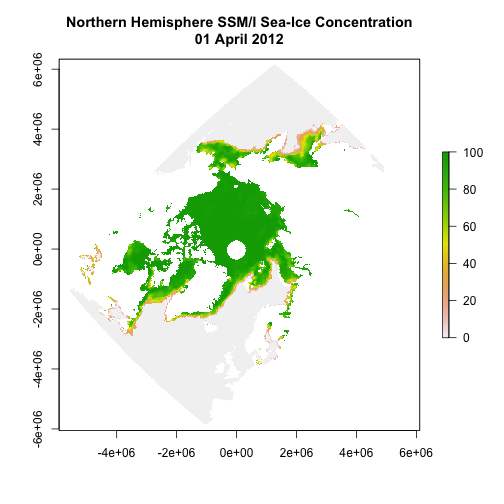
\includegraphics{figure/plot1.png}
\caption{plot of chunk plot1}
\end{figure}

Since the longitude of origin for this projection is 0 degrees, the map
is oriented with our region of interest (Bering Sea) upside down. To
resolve this, we'll use the \texttt{projectRaster} function to set the
latitude of origin to 180. We'll specify the same grid resolution
(25067.53 x 25067.53) and this should keep the raster aligned to the
original grid.

First, we will need to edit the PROJ.4 string to reflect this new
orientation

\begin{Shaded}
\begin{Highlighting}[]
\NormalTok{laea_180_proj <- }\KeywordTok{paste}\NormalTok{(}\StringTok{"+proj=laea +lat_0=90 +lon_0=180 +x_0=0 +y_0=0"}\NormalTok{, }
    \StringTok{"+datum=WGS84 +units=m +no_defs +ellps=WGS84 +towgs84=0,0,0"}\NormalTok{)}
\end{Highlighting}
\end{Shaded}
And, now, we'll re-project the raster and also re-project the
\emph{alaska\_dcw} and \emph{russia\_dcw} from the \texttt{nPacMaps}
package to this new projection

\begin{Shaded}
\begin{Highlighting}[]
\NormalTok{sic_raster <- }\KeywordTok{projectRaster}\NormalTok{(sic_raster, }\DataTypeTok{res =} \KeywordTok{c}\NormalTok{(}\FloatTok{25067.53}\NormalTok{, }\FloatTok{25067.53}\NormalTok{), }
    \DataTypeTok{crs =} \NormalTok{laea_180_proj)}
\KeywordTok{data}\NormalTok{(alaska_dcw)}
\KeywordTok{data}\NormalTok{(russia_dcw)}

\NormalTok{alaska_dcw <- }\KeywordTok{spTransform}\NormalTok{(alaska_dcw, }\KeywordTok{CRS}\NormalTok{(laea_180_proj))}
\NormalTok{russia_dcw <- }\KeywordTok{spTransform}\NormalTok{(russia_dcw, }\KeywordTok{CRS}\NormalTok{(laea_180_proj))}
\end{Highlighting}
\end{Shaded}
\begin{Shaded}
\begin{Highlighting}[]
\KeywordTok{plot}\NormalTok{(sic_raster, }\DataTypeTok{col =} \KeywordTok{colorRampPalette}\NormalTok{(}\KeywordTok{c}\NormalTok{(}\StringTok{"dark blue"}\NormalTok{, }\StringTok{"deepskyblue"}\NormalTok{, }
    \StringTok{"skyblue"}\NormalTok{, }\StringTok{"lightskyblue"}\NormalTok{, }\StringTok{"white"}\NormalTok{))(}\DecValTok{20}\NormalTok{), }\DataTypeTok{main =} \StringTok{"Northern Hempisphere SSM/I Sea-Ice Concentration}\CharTok{\textbackslash{}n}\StringTok{01 April 2012"}\NormalTok{)}
\KeywordTok{plot}\NormalTok{(alaska_dcw, }\DataTypeTok{add =} \OtherTok{TRUE}\NormalTok{)}
\KeywordTok{plot}\NormalTok{(russia_dcw, }\DataTypeTok{add =} \OtherTok{TRUE}\NormalTok{)}
\end{Highlighting}
\end{Shaded}
\begin{figure}[htbp]
\centering
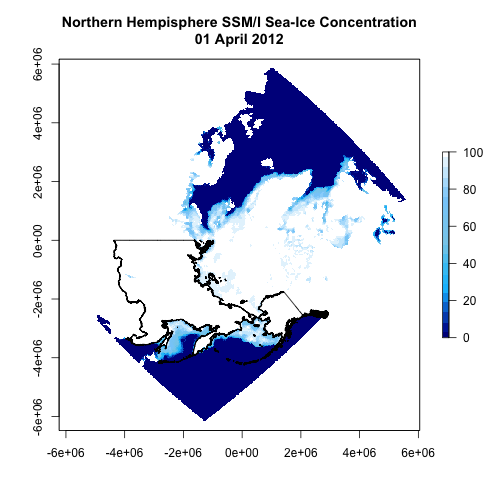
\includegraphics{figure/plot2.png}
\caption{plot of chunk plot2}
\end{figure}

For our purposes, we are only intersted in a sub-section of this grid.
The first thing needed is to establish an extent that defines the area
of interest. For this, we've settled on the following values:

\begin{Shaded}
\begin{Highlighting}[]
\NormalTok{x_min <- }\DecValTok{0}
\NormalTok{x_max <- }\DecValTok{1400000}
\NormalTok{y_min <- -}\DecValTok{3800000}
\NormalTok{y_max <- -}\DecValTok{1600000}
\end{Highlighting}
\end{Shaded}
And, then create an \emph{extent} object, we'll call \texttt{pep\_ext}

\begin{Shaded}
\begin{Highlighting}[]
\NormalTok{pep_ext <- }\KeywordTok{extent}\NormalTok{(x_min, x_max, y_min, y_max)}
\end{Highlighting}
\end{Shaded}
We can use the \texttt{crop} function within the \texttt{raster} package
to crop our \texttt{sic\_raster} to this extent. By specifying
``snap=`near'\,'', the function will snap the extent to the same grid as
\texttt{sic\_raster} prior to cropping.

\begin{Shaded}
\begin{Highlighting}[]
\NormalTok{sic_raster <- }\KeywordTok{crop}\NormalTok{(sic_raster, pep_ext, }\DataTypeTok{snap =} \StringTok{"near"}\NormalTok{)}
\NormalTok{pep_ext <- }\KeywordTok{extent}\NormalTok{(sic_raster)}
\end{Highlighting}
\end{Shaded}
\begin{Shaded}
\begin{Highlighting}[]
\KeywordTok{plot}\NormalTok{(sic_raster, }\DataTypeTok{col =} \KeywordTok{colorRampPalette}\NormalTok{(}\KeywordTok{c}\NormalTok{(}\StringTok{"dark blue"}\NormalTok{, }\StringTok{"deepskyblue"}\NormalTok{, }
    \StringTok{"skyblue"}\NormalTok{, }\StringTok{"lightskyblue"}\NormalTok{, }\StringTok{"white"}\NormalTok{))(}\DecValTok{20}\NormalTok{), }\DataTypeTok{main =} \StringTok{"SSM/I Sea-Ice Concentration and PEP BOSS Extent}\CharTok{\textbackslash{}n}\StringTok{01 April 2012"}\NormalTok{)}
\KeywordTok{plot}\NormalTok{(alaska_dcw, }\DataTypeTok{col =} \StringTok{"black"}\NormalTok{, }\DataTypeTok{add =} \OtherTok{TRUE}\NormalTok{)}
\KeywordTok{plot}\NormalTok{(russia_dcw, }\DataTypeTok{col =} \StringTok{"black"}\NormalTok{, }\DataTypeTok{add =} \OtherTok{TRUE}\NormalTok{)}
\KeywordTok{plot}\NormalTok{(pep_ext, }\DataTypeTok{col =} \StringTok{"red"}\NormalTok{, }\DataTypeTok{add =} \OtherTok{TRUE}\NormalTok{)}
\end{Highlighting}
\end{Shaded}
\begin{figure}[htbp]
\centering
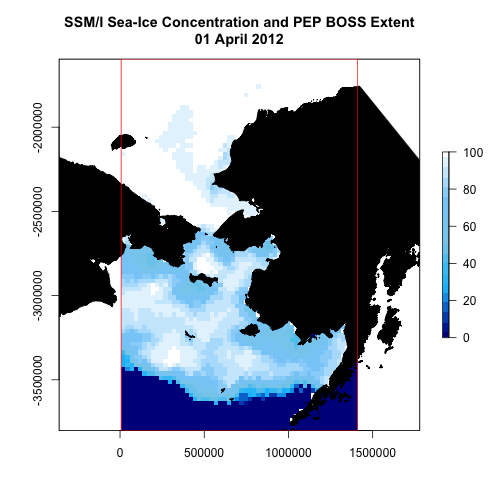
\includegraphics{figure/plot3.png}
\caption{plot of chunk plot3}
\end{figure}

\end{document}
